\documentclass{beamer}
\usepackage[utf8]{inputenc}
\usepackage{graphicx, epsfig}
\usepackage{amsmath,mathrsfs,amsfonts,amssymb}
%\usepackage{subfig}
\usepackage{floatflt}
\usepackage{epic,ecltree}
\usepackage{mathtext}
\usepackage{fancybox}
\usepackage{fancyhdr}
\usepackage{multirow}
\usepackage{enumerate}
\usepackage{epstopdf}
\usepackage{multicol}
\usepackage{algorithm}
\usepackage[noend]{algorithmic}
\usepackage{tikz}
\usepackage{blindtext}
\usetheme{default}%{Singapore}%{Warsaw}%{Warsaw}%{Darmstadt}
\usecolortheme{default}
\setbeamerfont{title}{size=\Huge}
\setbeamertemplate{footline}[page number]{}


\makeatletter
\newcommand\HUGE{\@setfontsize\Huge{35}{40}}
\makeatother    

\setbeamerfont{title}{size=\HUGE}
\beamertemplatenavigationsymbolsempty

% latin bold lower
\newcommand{\ba}{\mathbf{a}} 
\newcommand{\bc}{\mathbf{c}} 
\newcommand{\be}{\mathbf{e}} 
\newcommand{\bh}{\mathbf{h}} 
\newcommand{\bp}{\mathbf{p}} 
\newcommand{\bt}{\mathbf{t}} 
\newcommand{\bs}{\mathbf{s}} 
\newcommand{\bu}{\mathbf{u}} 
\newcommand{\bv}{\mathbf{v}} 
\newcommand{\bw}{\mathbf{w}} 
\newcommand{\bx}{\mathbf{x}} 
\newcommand{\by}{\mathbf{y}} 
\newcommand{\bz}{\mathbf{z}} 

% latin bold upper
\newcommand{\bA}{\mathbf{A}} 
\newcommand{\bB}{\mathbf{B}} 
\newcommand{\bC}{\mathbf{C}} 
\newcommand{\bI}{\mathbf{I}} 
\newcommand{\bL}{\mathbf{L}} 
\newcommand{\bM}{\mathbf{M}} 
\newcommand{\bQ}{\mathbf{Q}} 
\newcommand{\bT}{\mathbf{T}} 
\newcommand{\bU}{\mathbf{U}} 
\newcommand{\bV}{\mathbf{V}} 
\newcommand{\bW}{\mathbf{W}} 
\newcommand{\bX}{\mathbf{X}} 
\newcommand{\bY}{\mathbf{Y}} 
\newcommand{\bZ}{\mathbf{Z}} 

% latin cal upper
\newcommand{\cG}{\mathcal{G}} 
\newcommand{\cL}{\mathcal{L}} 
\newcommand{\cN}{\mathcal{N}} 
\newcommand{\cS}{\mathcal{S}} 
\newcommand{\cT}{\mathcal{T}} 
\newcommand{\cW}{\mathcal{W}} 
\newcommand{\cX}{\mathcal{X}} 
\newcommand{\cZ}{\mathcal{Z}} 

% latin bb upper
\newcommand{\bbE}{\mathbb{E}} 
\newcommand{\bbI}{\mathbb{I}} 
\newcommand{\bbP}{\mathbb{P}} 
\newcommand{\bbR}{\mathbb{R}} 

% greek bold lower
\newcommand{\bepsilon}{\boldsymbol{\epsilon}} 
\newcommand{\btheta}{\boldsymbol{\theta}} 
\newcommand{\blambda}{\boldsymbol{\lambda}} 
\newcommand{\bpi}{\boldsymbol{\pi}} 
\newcommand{\bmu}{\boldsymbol{\mu}} 
\newcommand{\bsigma}{\boldsymbol{\sigma}} 
\newcommand{\bphi}{\boldsymbol{\phi}} 

% greek bold upper
\newcommand{\bSigma}{\boldsymbol{\Sigma}} 

\DeclareMathOperator*{\argmin}{arg\,min}
\DeclareMathOperator*{\argmax}{arg\,max}

\newcommand{\createdgmtitle}[1]{\title[\hbox to 56mm{Deep Generative Models  \hfill\insertframenumber\,/\,\inserttotalframenumber}]
	{\vspace{1.5cm} \\ Deep Generative Models \\ {\Huge Lecture #1}}
	\author{Roman Isachenko}
	\institute{
	Moscow Institute of Physics and Technology
	} 
	\date{Autumn, 2021}
}

\newcommand\myfootnote[1]{%
  \tikz[remember picture,overlay]
  \draw (current page.south west) +(1in + \oddsidemargin,0.5em)
  node[anchor=south west,inner sep=0pt]{\parbox{\textwidth}{%
      \rlap{\rule{10em}{0.4pt}}\raggedright\scriptsize \textit{#1}}};}

\newcommand\myfootnotewithlink[2]{%
  \tikz[remember picture,overlay]
  \draw (current page.south west) +(1in + \oddsidemargin,0.5em)
  node[anchor=south west,inner sep=0pt]{\parbox{\textwidth}{%
      \rlap{\rule{10em}{0.4pt}}\raggedright\scriptsize\href{#1}{\textit{#2}}}};}
\createdgmtitle{6}
%--------------------------------------------------------------------------------
\begin{document}
%--------------------------------------------------------------------------------
\begin{frame}
%\thispagestyle{empty}
\titlepage
\end{frame}
%=======
\begin{frame}{Recap of previous lecture}
	\begin{figure}
		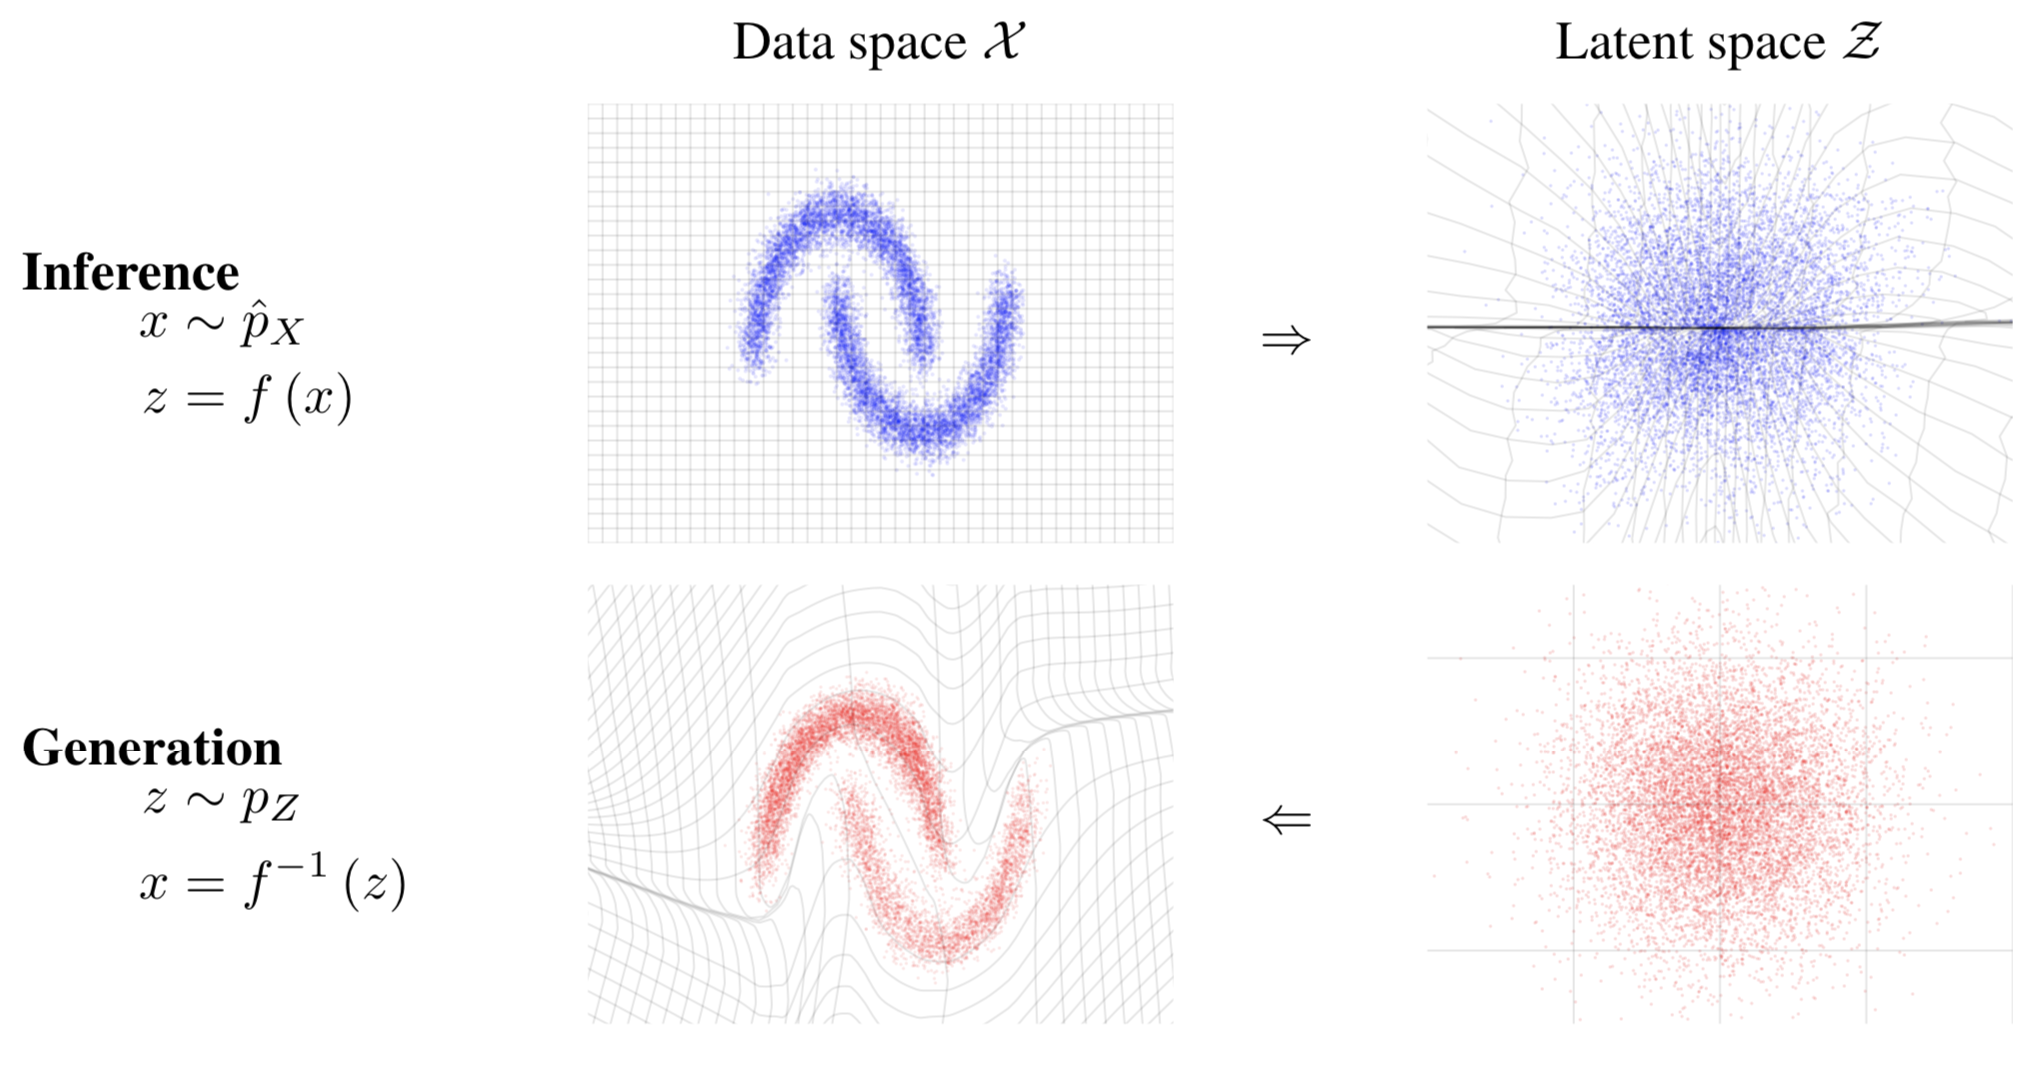
\includegraphics[width=0.7\linewidth]{figs/flows_how2.png}
	\end{figure}
	\vspace{-0.3cm}
		\begin{block}{Flow likelihood}
			\vspace{-0.3cm}
			\[
			\log p(\bx|\btheta) = \log p(f(\bx, \btheta)) + \log \left|\det \left( \frac{\partial f(\bx, \btheta)}{\partial \bx} \right) \right|
			\]
			\vspace{-0.5cm}
		\end{block}
		\begin{block}{What we want}
			\begin{itemize}
				\item Efficient computation of Jacobian $\frac{\partial f(\bx, \btheta)}{\partial \bx}$;
				\item Efficient sampling from the base distribution $p(\bz)$;
				\item Efficient inversion of $f(\bx, \btheta)$.
			\end{itemize}
			
		\end{block}
	\myfootnotewithlink{https://arxiv.org/abs/1605.08803}{Dinh L., Sohl-Dickstein J., Bengio S. Density estimation using Real NVP, 2016} 
\end{frame}
%=======
\begin{frame}{Recap of previous lecture}
	\vspace{-1.0cm}
	\begin{block}{Planar flow}
		\vspace{-0.5cm}
		\[
		g(\bz, \btheta) = \bz + \mathbf{u} \, h(\bw^T\bz + b).
		\]
		\vspace{-0.7cm}
	\end{block}
	\begin{block}{Sylvester flow}
		\vspace{-0.5cm}
		\[
			g(\bz, \btheta) = \bz + \bA \, h(\bB\bz + \mathbf{b}).
		\]
		\vspace{-0.7cm}
	\end{block}
	\begin{block}{NICE/RealNVP: Affine coupling law}
		\vspace{-0.3cm}
		\[
			\begin{cases} \bz_{1:d} = \bx_{1:d}; \\ \bz_{d:m} = \bx_{d:m} \odot \exp \left(c_1(\bx_{1:d}, \btheta)\right) + c_2(\bx_{1:d}, \btheta).\end{cases} 
		\]
		\vspace{-0.5cm}
	\end{block}
	\begin{block}{Glow: invertible 1x1 conv}
		\vspace{-0.3cm}
		\[
		\mathbf{W} = \mathbf{P}\mathbf{L}(\mathbf{U} + \text{diag}(\mathbf{s})).
		\]
	\end{block}
	\myfootnote{\href{https://arxiv.org/abs/1505.05770}{Rezende D. J., Mohamed S. Variational Inference with Normalizing Flows, 2015}\\
	\href{https://arxiv.org/abs/1803.05649}{Berg R. et al. Sylvester normalizing flows for variational inference, 2018} \\
	\href{https://arxiv.org/abs/1410.8516}{Dinh L., Krueger D., Bengio Y. NICE: Non-linear Independent Components Estimation, 2014} \\
	\href{https://arxiv.org/abs/1605.08803}{Dinh L., Sohl-Dickstein J., Bengio S. Density estimation using Real NVP, 2016} \\
	\href{https://arxiv.org/abs/1807.03039}{Kingma D. P., Dhariwal P. Glow: Generative Flow with Invertible 1x1 Convolutions, 2018}}
\end{frame}
%=======
\begin{frame}{Likelihood-based models}
\begin{block}{Exact likelihood evaluation}
	\begin{itemize}
		\item Autoregressive models (PixelCNN, WaveNet);
		\item Flow models (NICE, RealNVP, Glow).
	\end{itemize}
\end{block}
\begin{block}{Approximate likelihood evaluation}
	\begin{itemize}
		\item Latent variable models (VAE).
	\end{itemize}
\end{block}
What are the pros and cons of each of them? \\
\vspace{0.2cm}
\end{frame}
%=======
\begin{frame}{VAE recap}
\begin{block}{ELBO}
	\vspace{-0.3cm}
	\[
	\log p(\bx | \btheta) \geq \mathcal{L} (\bphi, \btheta)  = \mathbb{E}_{q(\bz | \bx, \bphi)} \log \frac{p(\bx, \bz | \btheta)}{q(\bz| \bx, \bphi)} \rightarrow \max_{\bphi, \btheta}.
	\]
	\vspace{-0.5cm}
\end{block}
\begin{figure}[h]
	\centering
	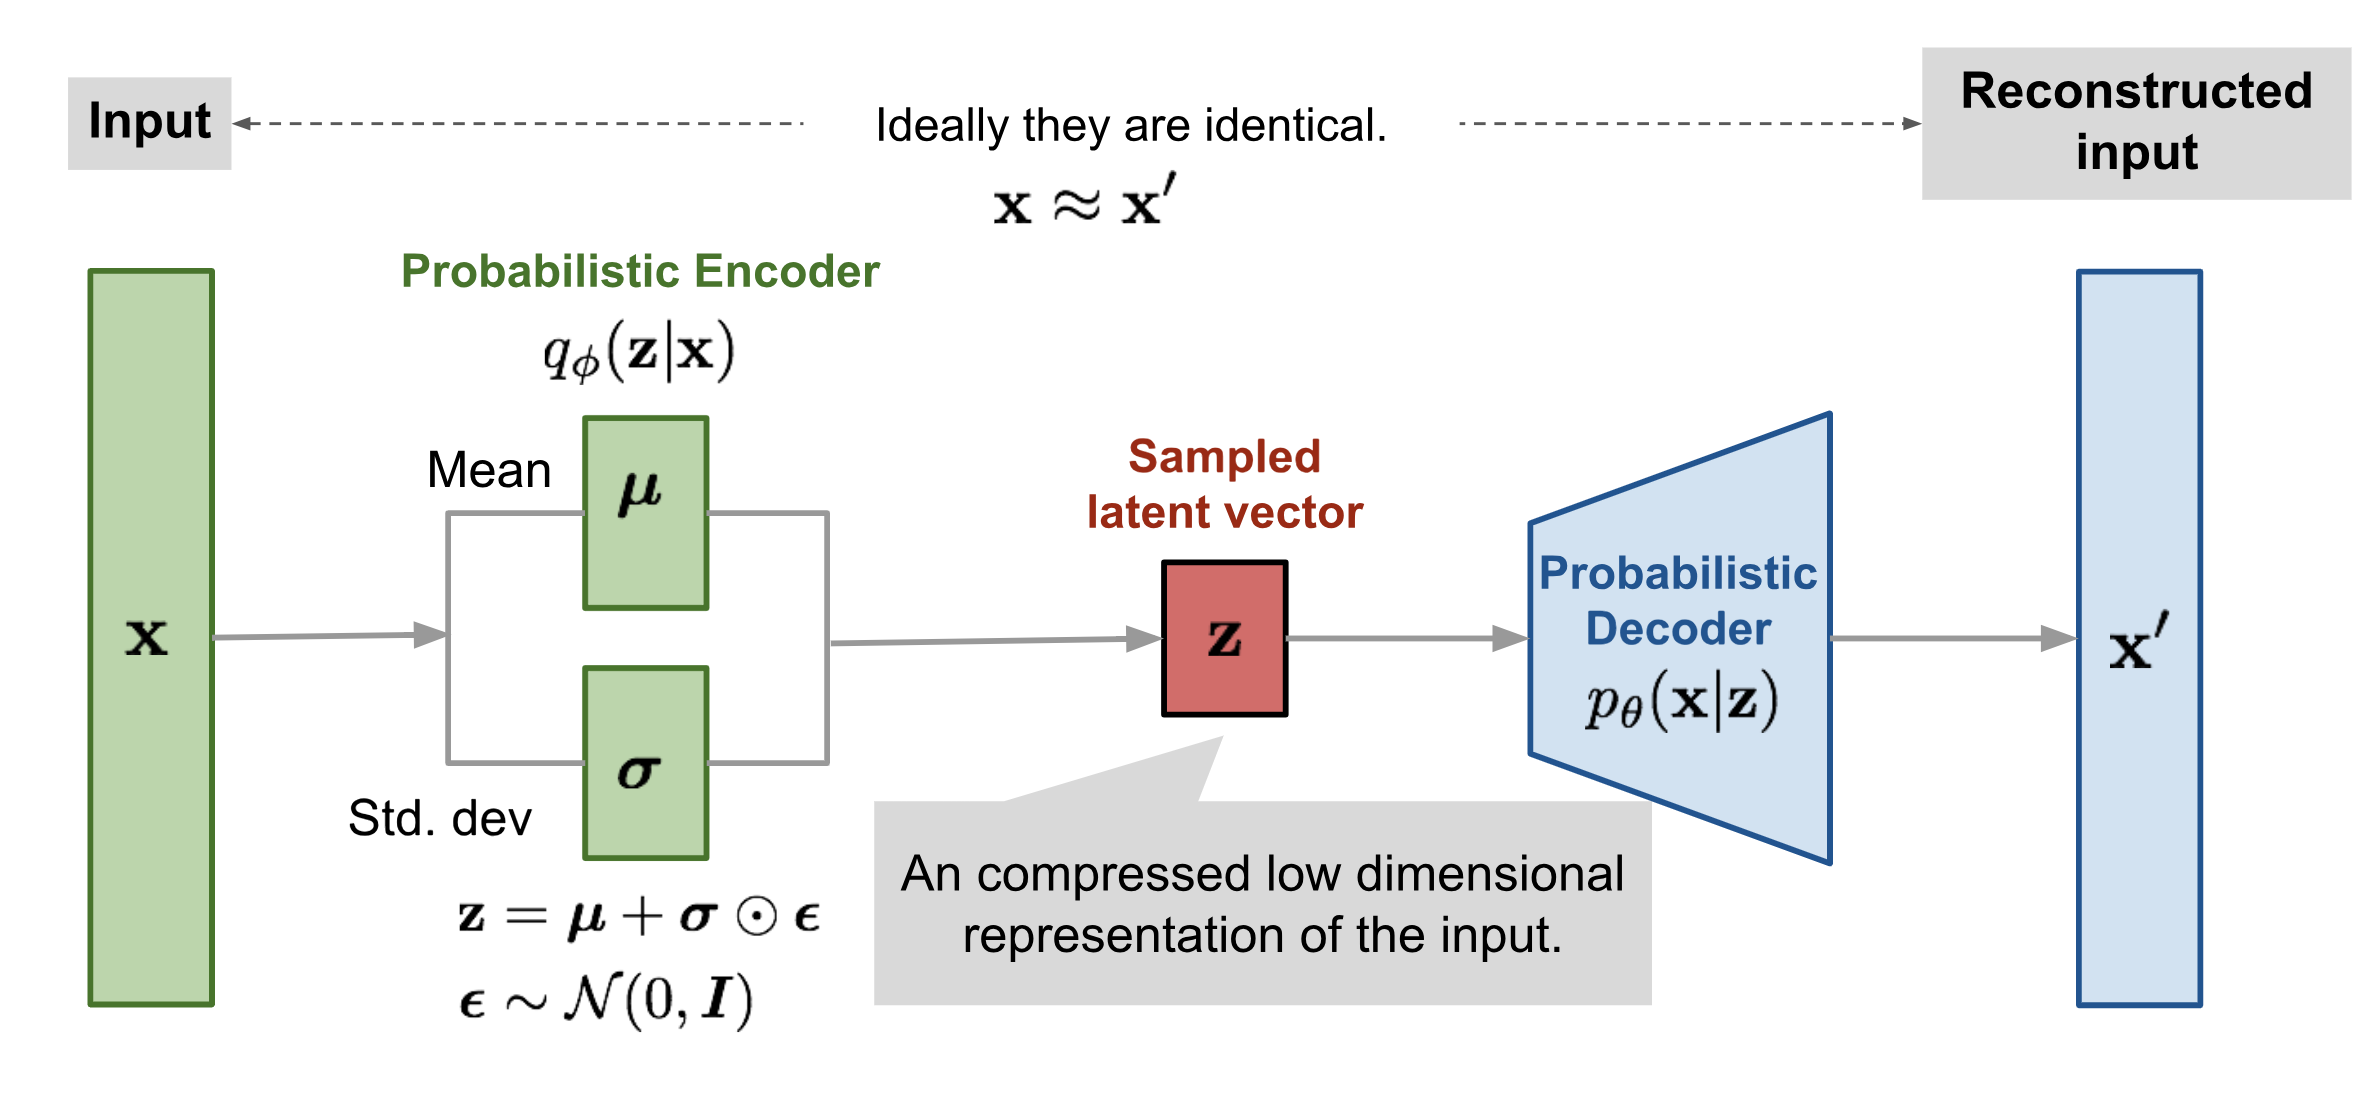
\includegraphics[width=\linewidth]{figs/vae-gaussian.png}
\end{figure}
\myfootnotewithlink{https://lilianweng.github.io/lil-log/2018/08/12/from-autoencoder-to-beta-vae.html}{image credit: https://lilianweng.github.io/lil-log/2018/08/12/from-autoencoder-to-beta-vae.html}

\end{frame}
%=======
\begin{frame}{VAE limitations}
\begin{itemize}
	\item Poor variational posterior distribution (encoder)
	\[
	q(\bz | \bx, \bphi) = \mathcal{N}(\bz| \bmu_{\bphi}(\bx), \bsigma^2_{\bphi}(\bx)).
	\]
	\item Poor prior distribution
	\[
	p(\bz) = \mathcal{N}(0, \mathbf{I}).
	\]
	\item Poor probabilistic model (decoder)
	\[
	p(\bx | \bz, \btheta) = \mathcal{N}(\bx| \bmu_{\btheta}(\bz), \bsigma^2_{\btheta}(\bz)) \quad (\text{or } \text{Softmax}(\pi(\bz))).
	\]
	\item Loose lower bound
	\[
	\log p(\bx | \btheta) - \mathcal{L}(q, \btheta) = (?).
	\]
\end{itemize}
\end{frame}
%=======
\begin{frame}{Variational posterior}
\begin{block}{ELBO}
	\[
	\log p(\bx | \btheta) = \mathcal{L}(q, \btheta) + KL(q(\bz | \bx, \bphi) || p(\bz | \bx, \btheta)).
	\]
\end{block}
\begin{itemize}
	\item In E-step of EM-algorithm we wish $KL(q(\bz | \bx, \bphi) || p(\bz | \bx, \btheta)) = 0$. \\
	(In this case the lower bound is tight $\log p(\bx | \btheta) = \mathcal{L}(q, \btheta)$). \\
	\item Normal variational distribution $q(\bz | \bx, \bphi) = \mathcal{N}(\bz| \bmu_{\bphi}(\bx), \bsigma^2_{\bphi}(\bx))$ is poor (e.g. has only one mode). \\
	\item Flows models convert a simple base distribution to a compex one using invertible transformation with simple Jacobian. How to use flows in VAE?
\end{itemize}
\end{frame}
%=======
\begin{frame}{Flows in VAE}
Apply a sequence of transformations to the random variable
\[
\bz_0 \sim q(\bz | \bx, \bphi) = \mathcal{N}(\bz| \bmu_{\bphi}(\bx), \bsigma^2_{\bphi}(\bx)).
\]
Here, $q(\bz | \bx, \bphi)$ (which is a VAE encoder) plays a role of a base distribution.
\[
\bz_0 \xrightarrow{g_1} \bz_1 \xrightarrow{g_2} \dots \xrightarrow{g_K} \bz_K, \quad \bz_K = g(\bz_0), \quad g = g_K \circ \dots \circ g_1.
\]
Each $g_k $ is a flow transformation (e.g. planar, coupling layer) parameterized by $\bphi_k$.
\begin{align*}
	\log q_K(\bz_K | \bx, \bphi, \{\bphi_k\}_{k=1}^K) &= \log q(\bz_0 | \bx, \bphi) \\ &- \sum_{k=1}^K \log \left| \det \left( \frac{\partial g_k(\bz_{k - 1}, \bphi_k)}{\partial \bz_{k-1}} \right) \right|.
\end{align*}

\myfootnotewithlink{https://arxiv.org/abs/1505.05770}{Rezende D. J., Mohamed S. Variational Inference with Normalizing Flows, 2015} 
\end{frame}
%=======
\begin{frame}{Flows in VAE}
\begin{block}{ELBO}
	\vspace{-0.3cm}
	\[
	p(\bx | \btheta) \geq \mathcal{L} (\bphi, \btheta)  = \mathbb{E}_{q(\bz | \bx, \bphi)} \log \frac{p(\bx, \bz | \btheta)}{q(\bz| \bx, \bphi)} \rightarrow \max_{\bphi, \btheta}.
	\]
	\vspace{-0.5cm}
\end{block}
\begin{block}{Flow model in latent space}
	\vspace{-0.7cm}
	\[
	\log q_K(\bz_K | \bx, \bphi_*) = \log q(\bz_0 | \bx, \bphi) - \sum_{k=1}^K \log \left| \det \left( \frac{\partial g_k(\bz_{k - 1}, \bphi_k)}{\partial \bz_{k-1}} \right) \right|.
	\]
	\vspace{-0.5cm}
\end{block}
Let use $q_K(\bz_K | \bx, \bphi_*), \, \bphi_* = \{\bphi, \bphi_1, \dots, \bphi_K\}$ as a variational distribution. Here $\bphi$~-- encoder parameters, $\{\bphi_k\}_{k=1}^K$~-- flow parameters.

\begin{itemize}
	\item Encoder outputs base distribution $q(\bz_0 | \bx, \bphi)$.
	\item Flow model $\bz_K = g(\bz_0, \{\bphi_k\}_{k=1}^K)$ transforms the base distribution $q(\bz_0 | \bx, \bphi)$ to the distribution $q_K(\bz_K | \bx, \bphi_*)$.
	\item Distribution $q_K(\bz_K | \bx, \bphi_*)$ is used as a variational distribution for ELBO maximization.
\end{itemize}

\myfootnotewithlink{https://arxiv.org/abs/1505.05770}{Rezende D. J., Mohamed S. Variational Inference with Normalizing Flows, 2015} 
\end{frame}
%=======
\begin{frame}{Flows in VAE}
\begin{block}{Flow model in latent space}
	\vspace{-0.7cm}
	\[
	\log q_K(\bz_K | \bx, \bphi_*) = \log q(\bz_0 | \bx, \bphi) - \sum_{k=1}^K \log \left| \det \left( \frac{\partial g_k(\bz_{k - 1}, \bphi_k)}{\partial \bz_{k-1}} \right) \right|.
	\]
	\vspace{-0.5cm}
\end{block}
\begin{block}{ELBO objective}
	\vspace{-0.5cm}
	\begin{align*}
		\mathcal{L} (\bphi, \btheta)  &= \mathbb{E}_{q_K(\bz_K | \bx, \bphi_*)} \log \frac{p(\bx, \bz_K | \btheta)}{q_K(\bz_K| \bx, \bphi_*)} \\
		&= \mathbb{E}_{q_K(\bz_K | \bx, \bphi_*)} \bigl[\log p(\bx, \bz_K | \btheta) - \log q_K(\bz_K| \bx, \bphi_*) \bigr] \\ 
		&=  \mathbb{E}_{q_K(\bz_K | \bx, \bphi_*)} \log p(\bx | \bz_K, \btheta) - KL (q_K(\bz_K| \bx, \bphi_*) || p(\bz_K)).
	\end{align*}
\end{block}
The second term in ELBO is reverse KL divergence. Planar flows was originally proposed for variational inference in VAE.
\myfootnotewithlink{https://arxiv.org/abs/1505.05770}{Rezende D. J., Mohamed S. Variational Inference with Normalizing Flows, 2015} 
\end{frame}
%=======
\begin{frame}{Flows in VAE}
\begin{block}{Variational distribution}
	\vspace{-0.5cm}
	\[
	\log q_K(\bz_K | \bx, \bphi_*) = \log q(\bz_0 | \bx, \bphi) - \sum_{k=1}^K \log \left| \det \left( \frac{\partial g_k(\bz_{k - 1}, \bphi_k)}{\partial \bz_{k-1}} \right) \right|.
	\]
	\vspace{-0.5cm}
\end{block}
\begin{block}{ELBO objective}
	\vspace{-0.5cm}
	\begin{align*}
		\mathcal{L} (\bphi, \btheta) 
		&= \mathbb{E}_{q_K(\bz_K | \bx, \bphi_*)} \bigl[\log p(\bx, \bz_K | \btheta) - \log q_K(\bz_K| \bx, \bphi_*) \bigr] \\
		&= \mathbb{E}_{q(\bz_0 | \bx, \bphi)} \left. \bigl[\log p(\bx, \bz_K | \btheta) - \log q_K(\bz_K| \bx, \bphi_*) \bigr]\right|_{\bz_K = g(\bz_0, \{\bphi_k\}_{k=1}^K)} \\
		&= \mathbb{E}_{q(\bz_0 | \bx, \bphi)} \bigg[\log p(\bx, \bz_K | \btheta) -  \log q(\bz_0 | \bx, \bphi ) + \\ & \quad  + \sum_{k=1}^K \log \left| \det \left( \frac{\partial g_k(\bz_{k - 1}, \bphi_k)}{\partial \bz_{k-1}} \right) \right| \bigg].
	\end{align*}
\end{block}
\myfootnotewithlink{https://arxiv.org/abs/1505.05770}{Rezende D. J., Mohamed S. Variational Inference with Normalizing Flows, 2015} 
\end{frame}
%=======
\begin{frame}{Flows in VAE}
\begin{block}{Variational distribution}
	\vspace{-0.6cm}
	\[
	\log q_K(\bz_K | \bx, \bphi_*) = \log q(\bz_0 | \bx, \bphi) - \sum_{k=1}^K \log \left| \det \left( \frac{\partial g_k(\bz_{k - 1}, \bphi_k)}{\partial \bz_{k-1}} \right) \right|.
	\]
	\vspace{-0.6cm}
\end{block}
\begin{block}{ELBO objective}
	\vspace{-0.7cm}
	\begin{align*}
		\mathcal{L} (\bphi, \btheta) 
		&= \mathbb{E}_{q(\bz_0 | \bx, \bphi)} \bigg[\log p(\bx, \bz_K | \btheta) -  \log q(\bz_0 | \bx, \bphi ) + \\ & \quad  + \sum_{k=1}^K \log \left| \det \left( \frac{\partial g_k(\bz_{k - 1}, \bphi_k)}{\partial \bz_{k-1}} \right) \right| \bigg].
	\end{align*}
	\vspace{-0.5cm}
\end{block}
\begin{itemize}
	\item Obtain samples $\bz_0$ from the encoder.
	\item Apply flow model $\bz_K = g(\bz_0, \{\bphi_k\}_{k = 1}^K)$.
	\item Compute likelihood for $\bz_K$ using the decoder, base distribution for $\bz_0$ and the Jacobian.
	\item We do not need inverse flow function, if we use flows in variational inference.
\end{itemize}
\myfootnotewithlink{https://arxiv.org/abs/1505.05770}{Rezende D. J., Mohamed S. Variational Inference with Normalizing Flows, 2015} 
\end{frame}
%=======
\begin{frame}{Recap of previous lecture}
	\begin{block}{ELBO}
		\vspace{-0.3cm}
		\[
			p(\bx | \btheta) \geq \mathcal{L} (\bphi, \btheta)  = \mathbb{E}_{q(\bz | \bx, \bphi)} \log \frac{p(\bx, \bz | \btheta)}{q(\bz| \bx, \bphi)} \rightarrow \max_{\bphi, \btheta}.
		\]
		\vspace{-0.5cm}
	\end{block}
		\begin{itemize}
			\item Normal variational distribution $q(\bz | \bx, \bphi) = \mathcal{N}(\bz| \bmu_{\bphi}(\bx), \bsigma^2_{\bphi}(\bx))$ is poor (e.g. has only one mode). \\
			\item Flows models convert a simple base distribution to a compex one using an invertible transformation with simple Jacobian. 
		\end{itemize}
	\begin{block}{Flow model in latent space}
		\vspace{-0.7cm}
		\[
			\log q_K(\bz_K | \bx, \bphi_*) = \log q(\bz_0 | \bx, \bphi) - \sum_{k=1}^K \log \left| \det \left( \frac{\partial g_k(\bz_{k - 1}, \bphi_k)}{\partial \bz_{k-1}} \right) \right|.
		\]
		\vspace{-0.5cm}
	\end{block}
	Let's use $q_K(\bz_K | \bx, \bphi_*), \, \bphi_* = \{\bphi, \bphi_1, \dots, \bphi_K\}$ as a variational distribution. Here, $\bphi$~-- encoder parameters, $\{\bphi_k\}_{k=1}^K$~-- flow parameters.
	
	\myfootnotewithlink{https://arxiv.org/abs/1505.05770}{Rezende D. J., Mohamed S. Variational Inference with Normalizing Flows, 2015} 
\end{frame}
%=======
\begin{frame}{Recap of previous lecture}
	\begin{block}{Variational distribution}
		\vspace{-0.6cm}
		\[
			\log q_K(\bz_K | \bx, \bphi_*) = \log q(\bz_0 | \bx, \bphi) - \sum_{k=1}^K \log \left| \det \left( \frac{\partial g_k(\bz_{k - 1}, \bphi_k)}{\partial \bz_{k-1}} \right) \right|.
		\]
		\vspace{-0.6cm}
	\end{block}
	\begin{block}{ELBO objective}
		\vspace{-0.7cm}
		\begin{align*}
			\mathcal{L} (\bphi, \btheta) 
			&= \mathbb{E}_{q(\bz_0 | \bx, \bphi)} \bigg[\log p(\bx, \bz_K | \btheta) -  \log q(\bz_0 | \bx, \bphi ) + \\ & \quad  + \sum_{k=1}^K \log \left| \det \left( \frac{\partial g_k(\bz_{k - 1}, \bphi_k)}{\partial \bz_{k-1}} \right) \right| \bigg].
		\end{align*}
		\vspace{-0.5cm}
	\end{block}
	\begin{itemize}
		\item Obtain samples $\bz_0$ from the encoder.
		\item Apply flow model $\bz_K = g(\bz_0, \{\bphi_k\}_{k = 1}^K)$.
		\item Compute likelihood for $\bz_K$ using the decoder, base distribution for $\bz_0$ and the Jacobian.
		\item We do not need an inverse flow function if we use flows in variational inference.
	\end{itemize}
	\myfootnotewithlink{https://arxiv.org/abs/1505.05770}{Rezende D. J., Mohamed S. Variational Inference with Normalizing Flows, 2015} 
\end{frame}
%=======
\begin{frame}{Inverse autoregressive flow (IAF)}
	\vspace{-0.3cm}
	\begin{align*}
		\bx &= g(\bz, \btheta) \quad \Rightarrow \quad x_i = \tilde{\sigma}_i (\bz_{1:i-1}) \cdot z_i + \tilde{\mu}_i(\bz_{1:i-1}). \\
		\bz &= f(\bx, \btheta) \quad \Rightarrow \quad z_i = \left(x_i - \tilde{\mu}_i(\bz_{1:i-1}) \right) \cdot \frac{1}{\tilde{\sigma}_i (\bz_{1:i-1})}.
	\end{align*}
	\vspace{-0.5cm}
	\begin{block}{Reverse KL for flow model}
  		\vspace{-0.5cm}
		\[
			KL(p || \pi)  = \bbE_{p(\bz)} \left[  \log p(\bz) - \log \left|\det \left( \frac{\partial g(\bz, \btheta)}{\partial \bz} \right) \right| - \log \pi(g(\bz, \btheta)) \right]
		\]
		\vspace{-0.3cm}
	\end{block}
	\begin{itemize}
	\item We don’t need to think about computing the function $f(\bx, \btheta)$.
	\item Inverse autoregressive flow is a natural choice for using flows in VAE:
	\end{itemize}
	\vspace{-0.3cm}
	\begin{align*}
		\bz_0 &= \bsigma(\bx) \odot \bepsilon + \bmu(\bx), \quad \bepsilon \sim \mathcal{N}(0, 1); \quad  \sim q(\bz_0 | \bx, \bphi). \\
		\bz_k &= \tilde{\bsigma}_k(\bz_{k - 1}) \odot \bz_{k-1} + \tilde{\bmu}_k(\bz_{k - 1}), \quad k \geq 1; \quad  \sim q_k(\bz_k | \bx, \bphi, \{\bphi_j\}_{j=1}^k).
	\end{align*}
	\myfootnotewithlink{https://arxiv.org/abs/1606.04934}{Kingma D. P. et al. Improving Variational Inference with Inverse Autoregressive Flow, 2016} 
\end{frame}
%=======
\begin{frame}{Inverse autoregressive flow (IAF)}
	\begin{figure}
		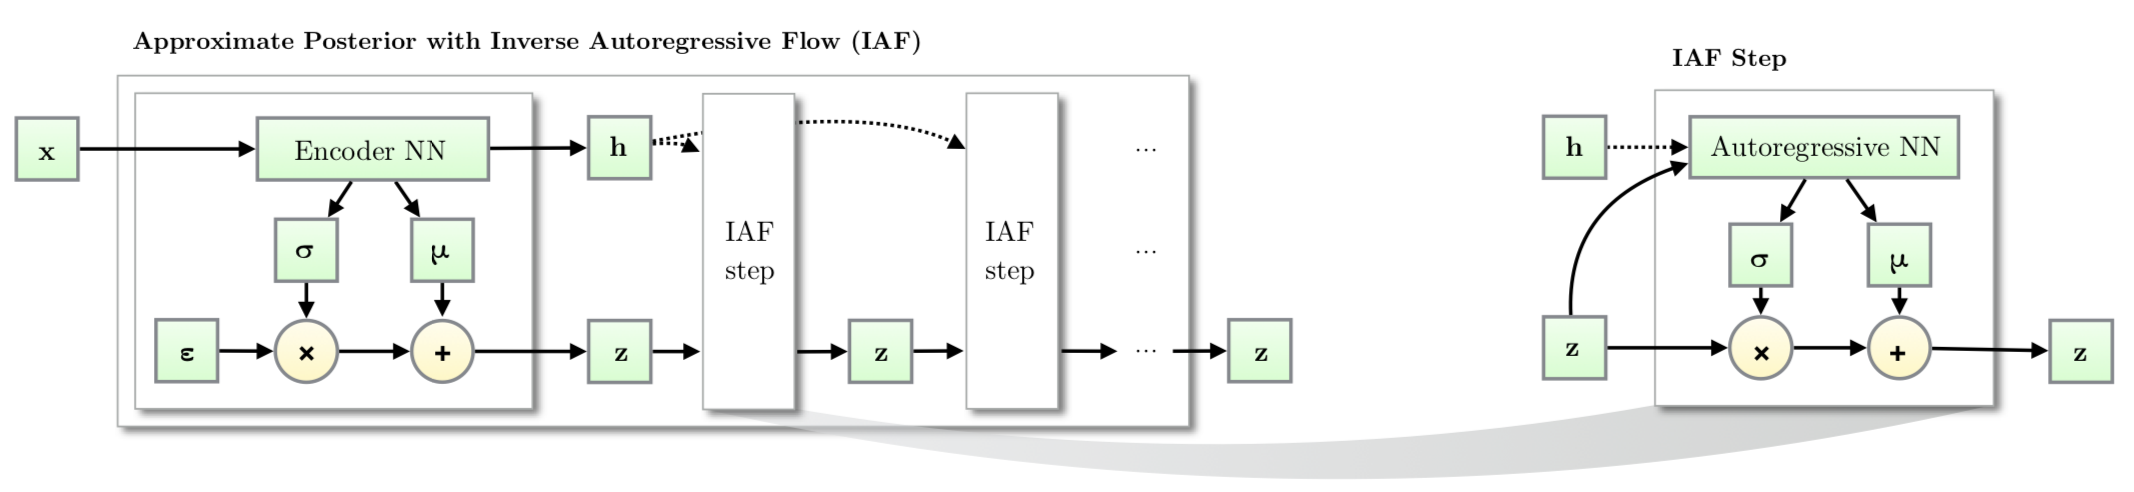
\includegraphics[width=\linewidth]{figs/iaf2.png}
	\end{figure}
	\begin{figure}
		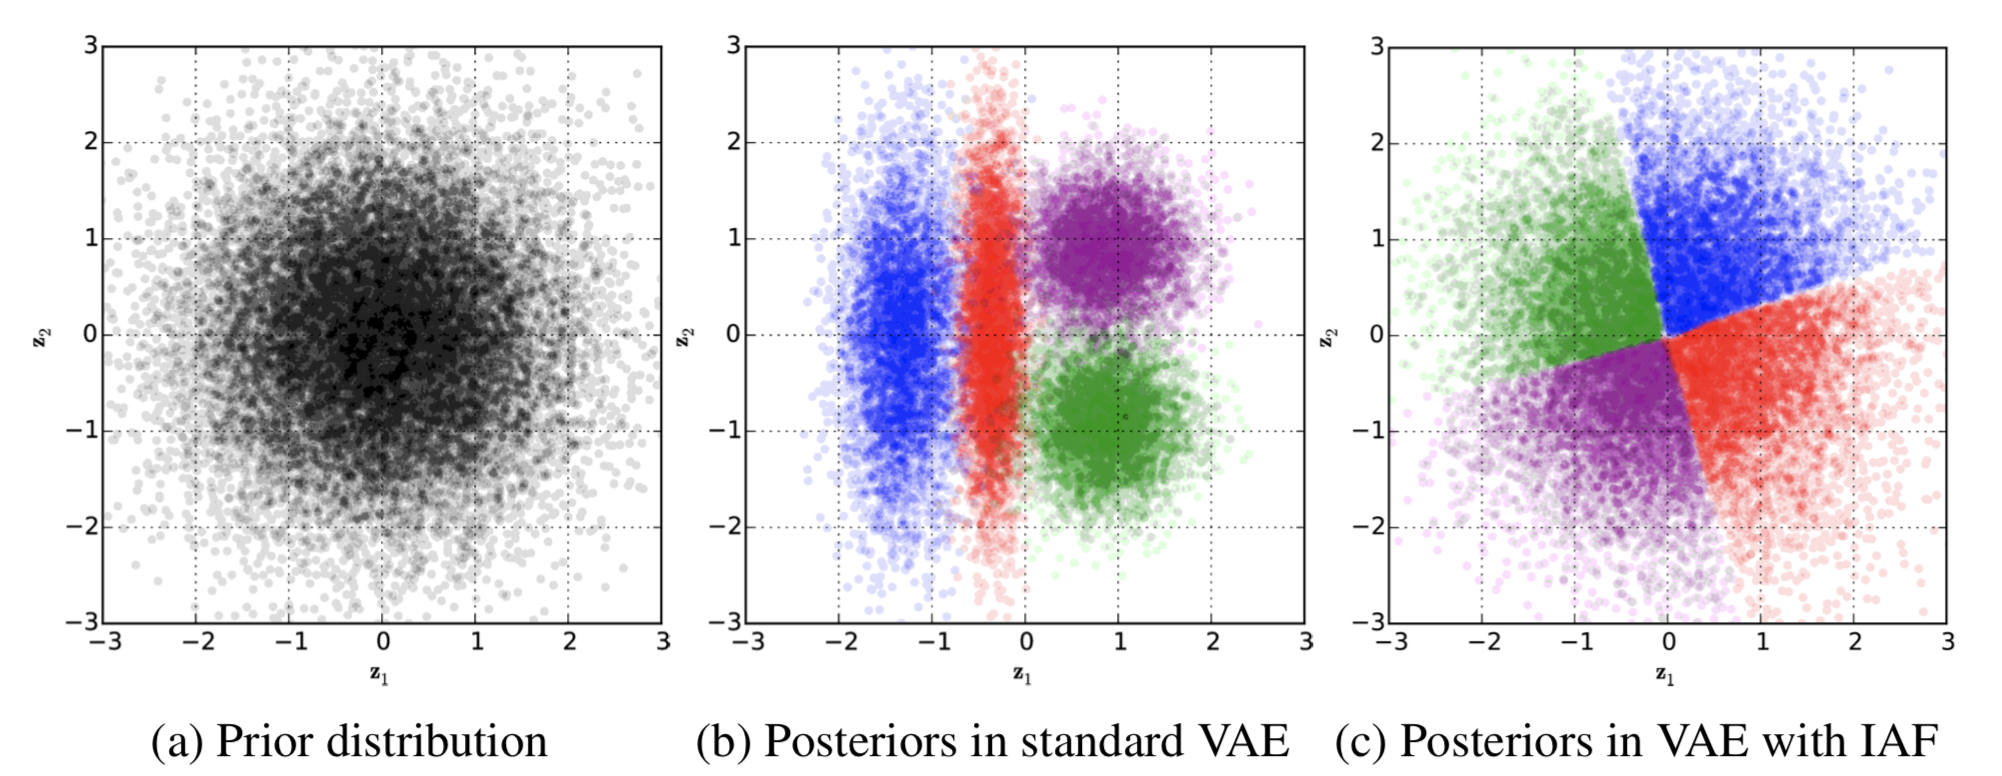
\includegraphics[width=\linewidth]{figs/iaf1.png}
	\end{figure}

	\myfootnotewithlink{https://arxiv.org/abs/1606.04934}{Kingma D. P. et al. Improving Variational Inference with Inverse Autoregressive Flow, 2016} 
\end{frame}
%=======
\begin{frame}{MAF/IAF pros and cons}
	\begin{block}{MAF}
		\begin{itemize}
			\item Sampling is slow.
			\item Likelihood evaluation is fast.
		\end{itemize}
	\end{block}
	\begin{block}{IAF}
		\begin{itemize}
			\item Sampling is fast.
			\item Likelihood evaluation is slow.
		\end{itemize}
	\end{block}
	\vspace{0.3cm}
	How to take the best of both worlds?
\end{frame}
%=======
\begin{frame}{WaveNet (2016)}
	Autoregressive model for raw audio waveforms generation
	\vspace{-0.2cm}
	\[
	p(\bx| \btheta) = \prod_{t=1}^T p(x_t|\bx_{1:t-1}, \btheta).
	\]
	\vspace{-0.2cm}
	The model uses causal dilated convolutions.
	\begin{figure}
		\centering
		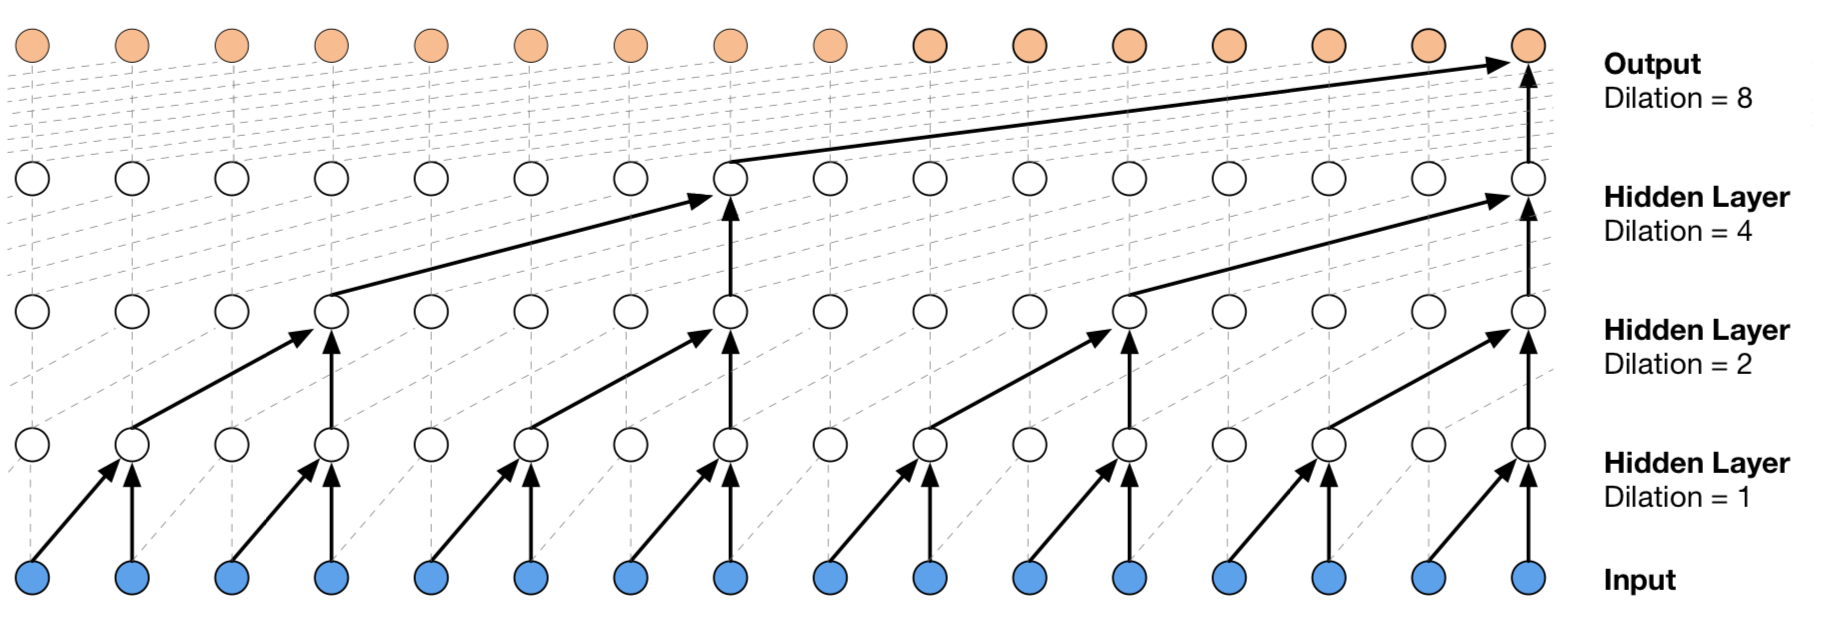
\includegraphics[width=0.9\linewidth]{figs/wavenet2.png}
	\end{figure}
	\myfootnotewithlink{https://arxiv.org/abs/1609.03499}{Oord A. et al. Wavenet: A generative model for raw audio, 2016}
\end{frame}
%=======
\begin{frame}{Parallel WaveNet, 2017}
	\begin{block}{Previous WaveNet model}
		\begin{itemize}
			\item raw audio is high-dimensional (e.g. 16000 samples per second for 16kHz audio);
			\item WaveNet encodes 8-bit signal with 256-way categorical distribution.
		\end{itemize}
	\end{block}
	\begin{block}{Goal}
		\begin{itemize}
			\item improved fidelity (24kHz instead of 16kHz) $\rightarrow$ increase dilated convolution filter size from 2 to 3;
			\item 16-bit signals $\rightarrow$ mixture of logistics instead of categorical distribution.
		\end{itemize}
	\end{block}
	\myfootnotewithlink{https://arxiv.org/abs/1711.10433}{Oord A. et al. Parallel WaveNet: Fast High-Fidelity Speech Synthesis, 2017}
\end{frame}
%=======
\begin{frame}{Parallel WaveNet, 2017}
	\begin{block}{Probability density distillation}
		\begin{enumerate}
			\item Train usual WaveNet (MAF) via MLE (teacher network).
			\item Train IAF WaveNet (student network), which attempts to match the probability of its own samples under the distribution learned by the teacher.
		\end{enumerate}
	\end{block}
	\begin{block}{Student objective}
		\[
		KL(p_s || p_t) = H(p_s, p_t) - H(p_s).
		\]
	\end{block}
	More than 1000x speed-up relative to original WaveNet!
	\myfootnotewithlink{https://arxiv.org/abs/1711.10433}{Oord A. et al. Parallel WaveNet: Fast High-Fidelity Speech Synthesis, 2017}
\end{frame}
%=======
\begin{frame}{Parallel WaveNet, 2017}
	\begin{figure}
		\centering
		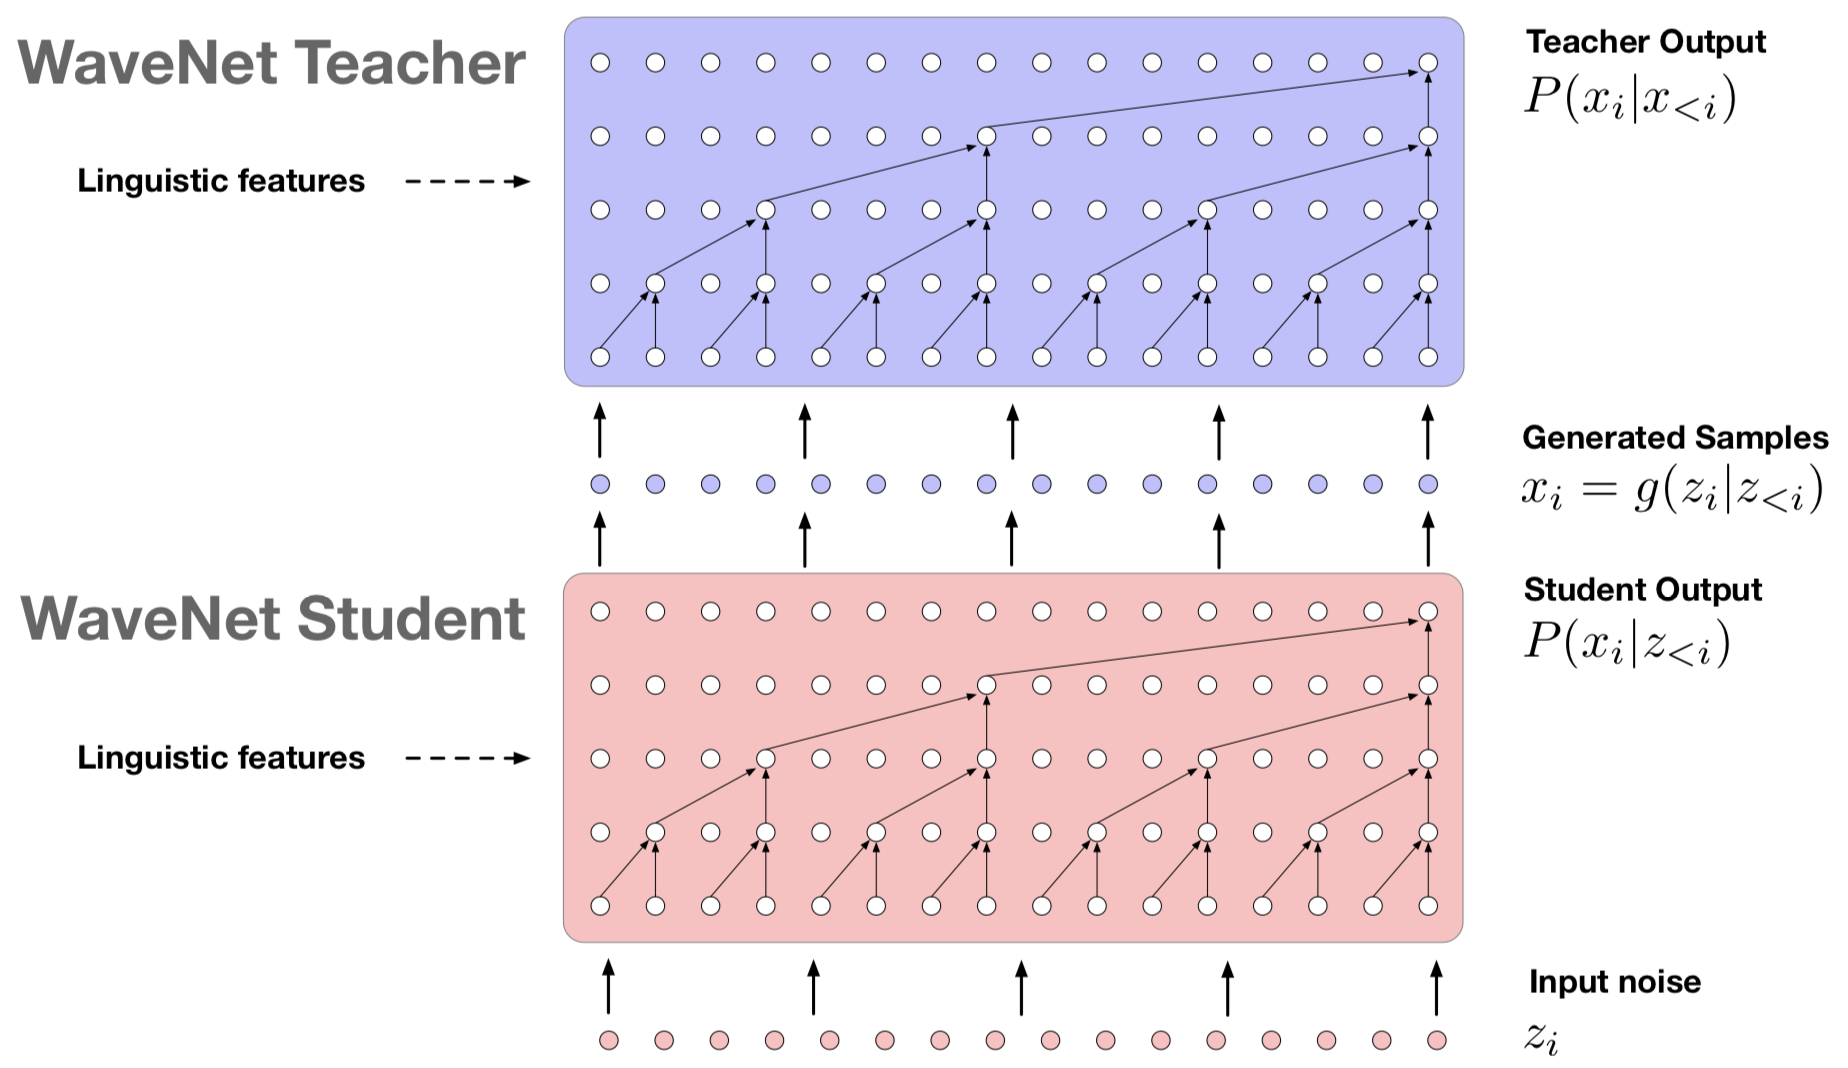
\includegraphics[width=\linewidth]{figs/parallel_wavenet.png}
	\end{figure}

	\myfootnotewithlink{https://arxiv.org/abs/1711.10433}{Oord A. et al. Parallel WaveNet: Fast High-Fidelity Speech Synthesis, 2017}
\end{frame}
%=======
\begin{frame}{Flow KL duality}
	\begin{block}{Theorem}
		Fitting flow model $p(\bx| \btheta)$ to the target distribution $\pi(\bx)$ using forward KL (MLE) is equivalent to fitting the induced distribution $p(\bz| \btheta)$ to the base $p(\bz)$ using reverse KL:
		\[
			\argmin_{\btheta} KL(\pi(\bx) || p(\bx | \btheta)) = \argmin_{\btheta} KL(p(\bz | \btheta) || p(\bz)).
		\]
		\vspace{-0.3cm}
		\begin{itemize}
			\item $p(\bz)$ is a base distribution; $\pi(\bx)$ is a data distribution;
			\item $\bz \sim p(\bz)$, $\bx = g(\bz, \btheta)$, $\bx \sim p(\bx| \btheta)$;
			\item $\bx \sim \pi(\bx)$, $\bz = f(\bx, \btheta)$, $\bz \sim p(\bz | \btheta)$;
		\end{itemize}
		\vspace{-0.3cm}
		\begin{align*}
			\log p(\bz | \btheta) &= \log \pi(g(\bz, \btheta)) + \log \left| \det \left( \frac{\partial g(\bz, \btheta)}{\partial \bz}\right) \right|; \\
			\log p(\bx | \btheta) &= \log p(f(\bx, \btheta)) + \log \left| \det \left( \frac{\partial f(\bx, \btheta)}{\partial \bx}\right) \right|.
		\end{align*}
	\end{block}
	\myfootnotewithlink{https://arxiv.org/abs/1912.02762}{Papamakarios G. et al. Normalizing flows for probabilistic modeling and inference, 2019} 
\end{frame}
%=======
\begin{frame}{MAF vs IAF}
	\begin{block}{Theorem}
		Fitting flow model $p(\bx| \btheta)$ to the target distribution $\pi(\bx)$ using forward KL (MLE) is equivalent to fitting the induced distribution $p(\bz| \btheta)$ to the base $p(\bz)$ using reverse KL:
		\[
			\argmin_{\btheta} KL(\pi(\bx) || p(\bx | \btheta)) = \argmin_{\btheta} KL(p(\bz | \btheta) || p(\bz)).
		\]
		\vspace{-0.5cm}
	\end{block}
	\begin{block}{Proof}
		\vspace{-0.5cm}
		\begin{multline*}
			KL\left(p(\bz | \btheta) || \pi(\bz) \right) = \mathbb{E}_{p(\bz | \btheta)} \bigl[ \log p(\bz | \btheta) - \log p(\bz) \bigr] = \\ 
			= \mathbb{E}_{p(\bz | \btheta)} \left[ \log \pi(g(\bz, \btheta)) + \log \left| \det \left( \frac{\partial g(\bz, \btheta)}{\partial \bz}\right) \right| - \log p(\bz) \right] = \\
			= \mathbb{E}_{\pi(\bx)} \left[ \log \pi(\bx) - \log \left| \det \left( \frac{\partial f(\bx, \btheta)}{\partial \bx}\right) \right| - \log p(f(\bx, \btheta)) \right].
		\end{multline*}
	\end{block}
	\myfootnotewithlink{https://arxiv.org/abs/1705.07057}{Papamakarios G., Pavlakou T., Murray I. Masked Autoregressive Flow for Density Estimation, 2017} 
\end{frame}
%=======
\begin{frame}{MAF vs IAF}
	\begin{block}{Theorem}
		Fitting flow model $p(\bx| \btheta)$ to the target distribution $\pi(\bx)$ using forward KL (MLE) is equivalent to fitting the induced distribution $p(\bz| \btheta)$ to the base $p(\bz)$ using reverse KL:
		\[
			\argmin_{\btheta} KL(\pi(\bx) || p(\bx | \btheta)) = \argmin_{\btheta} KL(p(\bz | \btheta) || p(\bz)).
		\]
		\vspace{-0.5cm}
	\end{block}
	\begin{block}{Proof (continued)}
		\vspace{-0.5cm}
		\begin{multline*}
			KL\left(p(\bz | \btheta) || p(\bz) \right) = \\
			=  \mathbb{E}_{\pi(\bx)} \left[ \log \pi(\bx) - \log \left| \det \left( \frac{\partial f(\bx, \btheta)}{\partial \bx}\right) \right| - \log p(f(\bx, \btheta)) \right] = \\
			= \mathbb{E}_{\pi(\bx)} \bigl[ \log \pi(\bx) - \log p(\bx | \btheta) \bigr] = KL (\pi(\bx) || p(\bx | \btheta)).
		\end{multline*}
	\end{block}
	\myfootnotewithlink{https://arxiv.org/abs/1705.07057}{Papamakarios G., Pavlakou T., Murray I. Masked Autoregressive Flow for Density Estimation, 2017} 
\end{frame}
%=======
\begin{frame}{Dequantization}
	\begin{itemize}
		\item Images are discrete data, pixels lie in the [0, 255] integer domain (the model is $P(\bx | \btheta) = \text{Categorical}(\bpi(\btheta))$).
		\item Flow is a continuous model (it works with continuous data $\bx$).
	\end{itemize}
	By fitting a continuous density model to discrete data, one can produce a degenerate solution with all probability mass on discrete values. \\
	How to convert a discrete data distribution to a continuous one?
	
	\begin{minipage}[t]{0.5\columnwidth}
		\begin{block}{Uniform dequantization}
		\vspace{-0.5cm}
			\begin{align*}
				\bx &\sim \text{Categorical}(\bpi) \\
				 \bu &\sim U[0, 1]
			\end{align*}
			\[
			\by = \bx + \bu \sim \text{Continuous} 
			\]
		\end{block}
	\end{minipage}%
	\begin{minipage}[t]{0.5\columnwidth}
		\begin{figure}
			\centering
			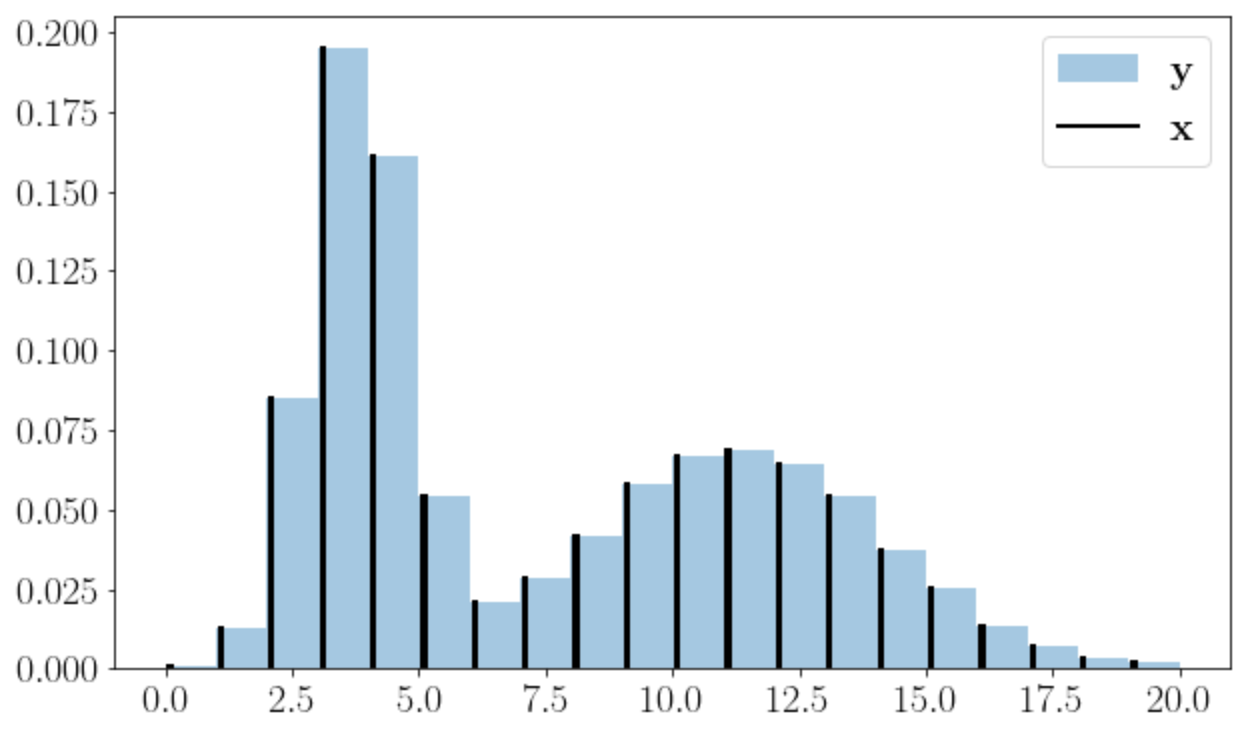
\includegraphics[width=1.0\linewidth]{figs/uniform_dequantization.png}
		\end{figure}
	\end{minipage}
	\myfootnotewithlink{https://arxiv.org/abs/1511.01844}{Theis L., Oord A., Bethge M. A note on the evaluation of generative models. 2015}
\end{frame}
%=======
\begin{frame}{Uniform dequantization}
	\begin{block}{Statement}
		Fitting continuous model $p(\by | \btheta)$ on uniformly dequantized data $\by = \bx + \bu, \, \bu \sim U[0, 1]$ is equivalent to maximization of a lower bound on log-likelihood for a discrete model:
		\[
		P(\bx | \btheta) = \int_{U[0, 1]} p(\bx + \bu | \btheta) d \bu
		\]
		\vspace{-0.2cm} \\
		Thus, the maximisation of continuous model log-likelihood on $\by$ can't lead to the a collapse onto the discrete data (the objective is bounded above by the discrete model log-likelihood).
	\end{block}
	\begin{block}{Proof}
		\vspace{-1cm}
		\begin{multline*}
			 \log P(\bx | \btheta) = \log \int_{U[0, 1]} p(\bx + \bu | \btheta) d \bu \geq \\ \geq \int_{U[0, 1]} \log p(\bx + \bu | \btheta) d \bu = \log p(\by | \btheta).
		\end{multline*}
	\end{block}
\end{frame}
%=======
\begin{frame}{Summary}
	\begin{itemize}
		\item Gaussian autoregressive model is a special type of flow.
		\vfill
		\item MAF is an example of such a model which is suitable for density estimation tasks. IAF uses an inverse autoregressive transformation for variational inference task.
		\vfill
		\item RealNVP is a special case of IAF and MAF.
		\vfill
		\item There is a duality between forward and reverse KL for flow models.
		\vfill
		\item To apply a continuous model to a discrete distribution it is standard practice to dequantize data at first.
	\end{itemize}
\end{frame}
%=======
\end{document} 